%\documentclass{article}
%\usepackage{tikz}
%\usepackage{scalefnt}
%\begin{document}

%\begin{figure}[h]
%\begin{center}

{\scalefont{0.8}
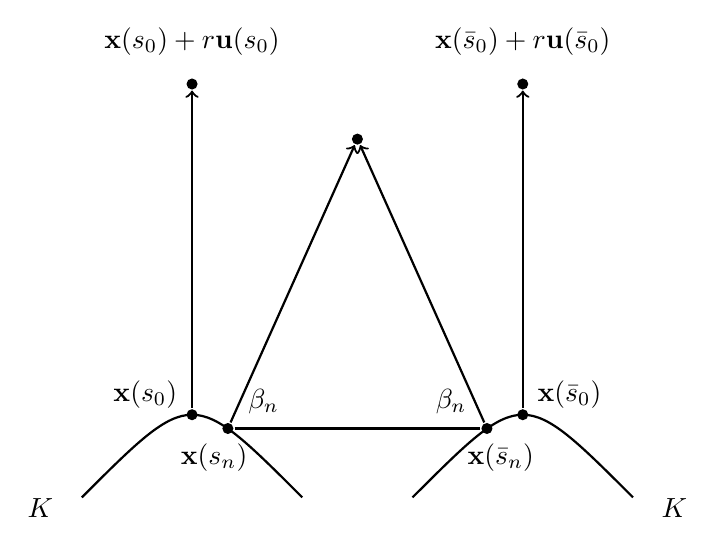
\begin{tikzpicture}[inner sep=0pt,thick,
        dot/.style={fill=black,circle,minimum size=4pt},scale=3.5]

\draw[thick] (0.2,0) .. controls (0.6,0.4) .. (1.0,0);
\draw[thick] (-0.2,0) .. controls (-0.6,0.4) .. (-1.0,0);

\node[dot](a) at (-0.6,0.3) {};
\node[above left](aa) at (-0.65,0.32){$\mathbf{x}(s_0)$};
\node[dot](b) at (0.6,0.3) {};
\node[above right](bb) at (0.65,0.32){$\mathbf{x}(\bar{s}_0)$};
\node[dot](c) at (-0.47,0.25) {};
\node[below](cc) at (-0.52,0.20){$\mathbf{x}(s_n)$};

\node[dot](d) at (0.47,0.25) {};
\node[below](cc) at (0.52,0.20){$\mathbf{x}(\bar{s}_n)$};
\node[above right](aaa) at (-0.4,0.3){$\beta_n$};
\node[above left](bbb) at (0.4,0.3){$\beta_n$};

\node[dot](e) at (0,1.3) {};
%\node[above](ee) at (0, 1.4) {$\gamma(s_n) + r(s_n, \bar{s}_n)\vec{u}(s_n)$};
%\node[above](eee) at (0, 1.4) {$= \gamma(\bar{s}_n) + r(s_n, \bar{s}_n)\vec{u}(\bar{s}_n)$};


\node[below left](ff) at (-1.1,0){$K$};
\node[below right](gg) at (1.1,0){$K$};

\draw (c) -- (d);
\draw[->] (c) -- (e);
\draw[->] (d) -- (e);


\node[dot](h) at (0.6,1.5) {};
\node[dot](i) at (-0.6,1.5) {};

\draw[->] (b) -- (h);
\draw[->] (a) -- (i);

\node[above](ii) at (-0.6,1.6) {$\mathbf{x}(s_0) + r\mathbf{u}(s_0)$};
\node[above](hh) at (0.6,1.6) {$\mathbf{x}(\bar{s}_0) + r\mathbf{u}(\bar{s}_0)$};




\end{tikzpicture}}

%\end{center}
%\caption{Schematic of Isosceles Triangles Formed Near Goal Post}
%\end{figure}

%\end{document}